\chapter{Related Work and Market Products}
\label{ch:SOTA}
This chapter takes a look at current literature in a similar area as well as existing companies developing products in this field.

%
% Section: State of the Art
%
\section{Current State of the Art}
\label{sec:sota:stateOfTheArt}
At the time of writing, research has yet to be conducted on how to mimic the functionality of cookies through cryptocurrency wallets and NFTs. There is an obvious research gap in this are. This paper attempts to fill that gap. 

Online Stores and NFTs / Wallets
How is user data typically tracked online? 
Are there already nfts, sites, and tools to track data using nfts? 
Challenge of high entry barrier with nfts and wallets. A lot of nec- essary know-how 


%
% Section: Related Work
%
\section{Related Work}
\label{sec:sota:relatedWork}
A plethora of relevant research has been conducted on cookies, including their privacy issues, and on wallets and NFTs. This paper aims to bring these two areas of research together to answer the question at hand.

% Cookies
\subsection{Cookies}
\label{sec:sota:cookies}
Todo

% NFTs and Web3
\subsection{NFTs, Wallets, and Web3}
\label{sec:sota:nfts}
Todo



%
% Section: Current Market Products
%
\section{Current Market Products}
\label{sec:sota:products}
Within the realm of this research, no company was found that openly speaks about acquiring data through wallets in order to learn more about their users. However, there are a handful of companies and products that make it possible to do so.

The following companies and products support the case study  of this paper (as will be mentioned in more detail later in section \ref{sec:methodology:caseStudy}).

Especially relevant for this paper is any type of application or product that allows SSO for a dApp using a user's wallet. SSO works by replacing the typical username and password login. Instead, a single ID such as your Google account can be used to login across all websites that support a Google login. This can also be done with a cryptocurrency wallet, so long as the wallet offers an API for developers to create a SSO with it on their website.

% Meta Mask
\subsection{MetaMask}
\label{sec:sota:metaMask}
MetaMask is a popular browser extension which works on most major browsers. It is a digital wallet and allows for interaction with the blockchain and dApps. With the extension installed, a user can use their wallet to sign in to any dApp that utilizes MetaMask's SSO. \cite{metaMask}

Figure \ref{fig:metamaskPopup} displays MetaMask's popup, when a website requests to connect to your wallet. As can be seen in the figure, the user's public address (0xd4c...) is displayed. With just this information, a plethora of information can be gathered on the user. The website is also requesting to see the wallet's account balance, activity, and will request transactions (which the user will manually have to accept or decline).

\begin{figure}[t]
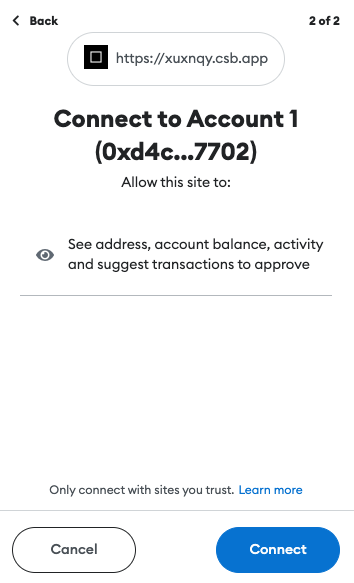
\includegraphics[width=8cm]{./gfx/metamaskPopup.png}
\centering
\caption{MetaMask's popup screen when a website requests to connect to a user's wallet.}
\label{fig:metamaskPopup}
\end{figure}


% Wallet Connect
\subsection{Wallet Connect}
\label{sec:sota:walletConnect}
Wallet Connect \cite{walletConnect} is a company developing various open source products which allow dApps to connect to your wallet. At the time of writing, their portfolio includes 4 products. However, only the \textit{Sign} product is so far released to the public.

\begin{itemize}
	\item Sign: A secure way to connect your wallet to dApps and make secure transactions between them. \cite{walletConnect}
	\item Auth: An SSO which works by connecting your wallet to dApps. This means that a user does not have to create an individual account for each platform. This is similar to MetaMask. \cite{walletConnect}
\end{itemize}
